%!TEX TS-program = xelatex
%!TEX encoding = UTF-8 Unicode
%!TEX root = 2024-gs-adonis-template.tex
%
\documentclass{gs-adonis}
\usepackage[english,italian]{babel}
%-------------------------------------------------------------------------------
%--------------------------------------------------------------------- CUSTOMS -
%-------------------------------------------------------------------------------
% \usepackage{showframe}
% \renewcommand\ShowFrameLinethickness{0.15pt}
% \renewcommand*\ShowFrameColor{\color{red}}
% %
% \usepackage{tikz}
% \usetikzlibrary{
%   shapes,
%   through,
%   calc,
%   intersections,
%   backgrounds,
%   positioning,
%   decorations.text
%   }
% \usetikzlibrary{arrows.meta}
% \usetikzlibrary{bending}
\usepackage[
  small,
  labelfont=bf,
  up,
  textfont=it,
  up
  ]{caption}
%
\usepackage{paralist}
\usepackage{subfigure}
%\usepackage{glossaries}
%\input{includes/glossario.tex}
%\makeglossaries
\usepackage{csquotes}
\usepackage[style=ieee,backend=biber]{biblatex}
\bibliography{includes/bibliografia.bib}
\usepackage{enumitem}
\usepackage{adjustbox}
\usepackage{hhline}
\DeclareLabelname[movie]{
    \field{director}
    \field{producer}
  }
\usepackage{scrextend}
\usepackage{calc}
\usepackage{mwe}

\usepackage{todonotes}
\usepackage{hyperref}
%-------------------------------------------------------------------------------
%------------------------------------------------------------------------ MAIN -
%-------------------------------------------------------------------------------
\title{Autocostruzione di un interprete.\\
       Per quale musica?}
\subtitle{sottotitolo?}
\author{Alice Cortegiani \textsuperscript{1}}
% secondary details
%\affiliation{\textsuperscript{1} Spherical Technologies SRLS}
\correspondence{alicecortegiani@gmail.com}
\version{\today}
% headers
\runningauthor{Alice Cortegiani}
\runningtitle{Autocostruzione di un interprete. Per quale musica?}
%-------------------------------------------------------------------------------
%--------------------------------------------------------------------- COMANDI -
%-------------------------------------------------------------------------------
% \newcommand{\studi}{\emph{Sei studi di Agamotto sul Tempo}}
% \newcommand{\tempo}{\emph{Tempo}}
% \newcommand{\canto}{\emph{canto alla durata}}
%-------------------------------------------------------------------------------
%-------------------------------------------------------------------- ABSTRACT -
%-------------------------------------------------------------------------------
\abstract{%
  %\begin{addmargin*}[0pt]{-\marginparsep-\marginparwidth}
  \input{includes/abstract.txt}
  %\end{addmargin*}
}
%-------------------------------------------------------------------------------
%-------------------------------------------------------------------- DOCUMENT -
%-------------------------------------------------------------------------------
\begin{document}
\maketitle
%\input{includes/000-citazioni.tex}
%
%\clearpage
%-------------------------------------------------------------------------------
%--------------------------------------------------------------------- APPUNTI -
%-------------------------------------------------------------------------------
% \section*{APPUNTI}
% \begin{compactitem}
%   \item questione etica
%   \item diagrammi a blocchi
%   \item storia di una ricerca, fagioli, sogno, immagine
%   \item rappresentazione
%   \item feedback
%   \item interfaccia
%   \item tecnica
%   \item musica
%   \item invenzione
%   \item{bibliografia da compilare:}
%   \begin{compactitem}
%     \item Bergson
%     \item Barthes
%     \item Borges
%     \item Branchi
%     \item Cacciari
%     \item Candiani
%     \item Di Scipio
%     \item Galante
%     \item Guaccero
%     \item Handke
%     \item Ferraris
%     \item Lupone
%     \item Netti
%     \item Nono
%     \item Ronchi
%     \item Sartre
%   \end{compactitem}
% \end{compactitem}
%
%\clearpage
%-------------------------------------------------------------------------------
%--------------------------------------------------------------------- APPUNTI -
%-------------------------------------------------------------------------------
%\tableofcontents
%\clearpage
%-------------------------------------------------------------------------------
%-------------------------------------------------------------------- INCLUDES -
%-------------------------------------------------------------------------------
% \input{includes/000-introduzione.tex}
% \input{includes/100-ciclobase.tex}
% \input{includes/200-cad.tex}
% \input{includes/300-tempo.tex}

% \clearpage
%
% \tiny
% \twocolumn
% \printglossary[title={glossarietto}]
%
% \clearpage

%\normalsize
%\onecolumn

\section{Key words}

[massimo 5 key words]


\section{Descrizione del progetto di ricerca}% (massimo 2.000 parole / 2.000 words)}

\subsection{1. Descrizione del soggetto di ricerca}% (600 parole):}

\emph{a) descrivere l’ambito generale e lo stato dell’arte della pratica musicale in cui e attraverso cui si desidera svolgere il proprio progetto;}

% #### SUONO, RUMORE, TIMBRO

% Il suono, nella sua infinita varietà e complessità, rappresenta un universo
% ancora non completamente esplorato. La musica, in particolare, offre un terreno
% fertile per indagare le profonde connessioni tra suono, sensazione e significato.

La ricerca sul suono, nelle possibilità individuabili attraverso la ricerca
musicale, nell'articolazione delle peculiarità di cui dispone, determina
l'ambito generale in cui il progetto si inscrive tracciando percorsi unici e di
indipendenza dalla ricerca scientifica e universitaria. I luoghi della ricerca,
i soggetti coinvolti e gli oggetti individuati sono accessibili e attivi solo
in un processo musicale.

L'ambito generale in cui il progetto si inscrive è quello della musica di
ricerca che, con radici profonde nei piccoli laboratori sperimentali del
novecento, oggi è fortemente rappresentato da centri di ricerca storici e
nuovi laboratori indipendenti, la cui attività musicale si riversa nella
pratica, nella didattica e nella divulgazione musicale a piu livelli. Questo
livello di contro-reazione (feedback) è possibile solo in condivisione di un
processo musicale mediante l'ascolto.

% Questa tematica di ricerca si propone di inve- stigare le molteplici sfaccettature
% della creazione, manipolazione e percezione timbrica in contesti musicali.

Il progetto si struttura attraverso le relazioni tra opera, strumento,
interprete mediante indagini di analisi e scrittura dove lo strumento definisce
la consapevolezza verso un pensiero creativo con la sua relativa prassi, non
incline a fini prestabiliti ma in continua tendenza verso presupposti utopici.
In ascolto.

Il progetto è inserito in una pratica quotidiana di ricerca presso laboratori
e centri specializzati.

Lo stato dell'arte della pratica musicale da cui il progetto è scalfito, pone,
ad un fare musicale attento,la necessità di un pensare creativo e analitico il
ruolo dell'interprete, poiché attraverso gli esiti dall'alta (de)formazione
artistica, facilmente si confonde la figura dell'esecutore con il ruolo
dell'interprete, precludendo così fondamentali contributi nel campo della
ricerca musicale, di un fare musicale condiviso, consumato nel fine
prestabilito dal dominio dell'intrattenimento.

\begin{figure}[ht]
  \centering
  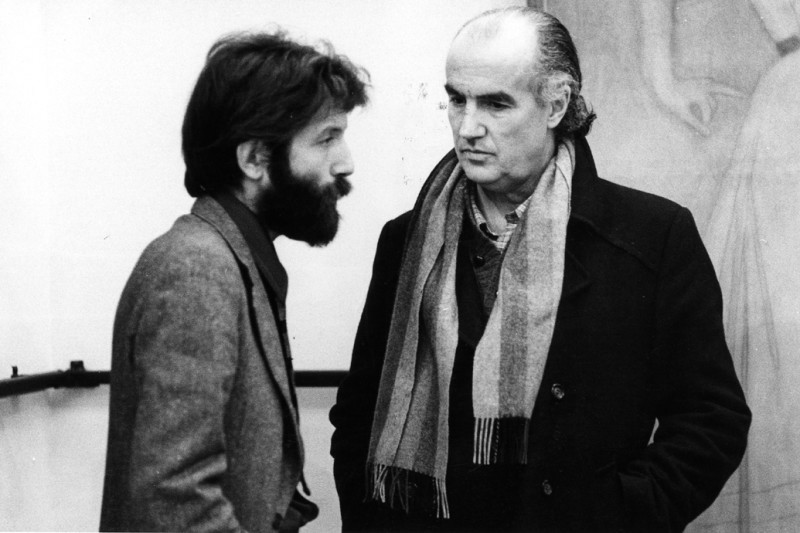
\includegraphics[width=\linewidth]{images/luigi-nono-massimo-cacciari.jpg}
  \captionsetup{width=.81\linewidth}
  \caption{Masimo Cacciari, Luigi Nono.}
  \label{cacciari}
\end{figure}


\emph{b) formulare il problema e una o più domande di ricerca relative ad esso che possano guidare l’esplorazione dell’argomento.}

\emph{Che cos'è un interprete?}

Massimo Cacciari nel descrivere il tema dell'ascolto in Luigi Nono \cite{Cacciari1995} disegna lo sfondo di una problematica filosofica che assale
la cultura occidentale nelle relazioni tra scrittura-voce-ascolto. Problemi di ordine generale che si riferiscono al significato culturale generale della nascita della scrittura alfabetica e che in un lento processo vede il dominio della visione sull'ascolto in una

\begin{quote}
progressiva desomatizzazione della voce. Una perdita dell'udire. L'udire
non è più una funzione fondamentale del comprendersi. \cite{Cacciari1995}
\end{quote}

Cacciari sottolinea che in molte pratiche artistiche questo problema può essere
dimenticato, può non essere un problema, ma non nella musica: la musica non può
essere senza ascolto. La perdita della memoria, dell'ascolto, della memoria
dell'ascolto è fatale per la musica. Questo accade perchè ad ogni ascolto muta
il testo stesso. La musica non può esistere senza un ascolto vivente, attivo.

In questo quadro di sensibilità musicale, l'interprete per primo, cercando di
comprendere, di capire che vorrebbe riuscire a comprendere di più ciò che c'è
\emph{prima del primo suono e dopo l'ultimo suono} \cite{Cacciari1995}, si fa
testimone della ricerca musicale nel luogo sonoro in cui opera in grado di
\emph{articolare, accentuare, dare al canto}, il testo musicale: a chiarire
anche la distanza dall'esecutore \emph{l'interprete non legge} il testo
musicale, \emph{lo riattiva, lo da al canto} \cite{Cacciari1995}.

Intraprendere il percorso di interprete nella musica contemporanea di ricerca è
un atto che conduce inevitabilmente all'individuazione di problemi nel campo
della formazione accademica, basata sul repertorio.

\emph{Che cos'è il repertorio?}

I programmi di studio dei corsi strumentali adottati dai conservatori di musica italiani favoriscono un percorso formativo
fondato sul repertorio d'intrattenimento, cristallizzando la sensibilità del musicista in una prassi parziale resa assoluta,
quindi distorta.
Riconoscere la pluralità del repertorio è elemento essenziale per avere accesso, dalla teoria,
alla complessità dei linguaggi musicali strutturati.
La prassi del repertorio di musica contemporanea di ricerca costruisce e si costituisce nel processo;
attraverso lo strumento acustico, strumento di pensiero, l'interprete è anello attivo della catena, generato e generatore.

Nel dominio dell'intrattenimento la chiave di lettura tende, sovente, erroneamente a sottovalutare aspetti fondamentali di apporto storico-sociale
che hanno nutrito la creazione musicale, favorendo ambizione e gratificazione nel risultato alla riproduzione del testo scritto.
Reperire, trovare, partecipare al processo creativo di musica contemporanea di ricerca comporta un costante confronto:
con le domande fondamentali di cui si nutre la prassi interpretativa, con gli strumenti da costruire per avere accesso al dialogo con
interlocutori dediti ad pensiero in ascolto, volti alla creazione e quindi nel reperire opere di ricerca dal pensiero musicale.

\emph{Che cos'è contemporaneo?}

\begin{quote}
  Contemporaneo è colui che riceve in pieno viso il fascio di tenebra che proviene dal suo tempo. \cite{agamben2008che}
\end{quote}

La contemporaneità è quindi un momento mobile del tempo che identifica la
facoltà di osservare l’oscurità del tempo specifico, quella relazione col
tempo che aderisce a esso attraverso una sfasatura e un anacronismo che ci
permette di valutare, vedere ed analizzare, alla dovuta distanza. Distanza da
cosa?

Fare repertorio contemporaneo, nella contemporaneità, nell’espressione del suo
senso più completo è imparare ad ascoltare.

Che cos'è la ricerca musicale contemporanea e come può formarsi l'interprete
contemporaneo?

\subsection{2. Metodi e processo di ricerca (600 parole):}

\emph{a) descrivere cosa si intende fare in termini pratici per indagare il proprio argomento di ricerca;}

Autocostruzione… citazione Mari.

\emph{lo studio delle proprietà fisiche e psicoacustiche che definiscono il timbro di un determinato strumento, di una voce o di un suono complesso;}

\emph{sperimentazione nella propria pratica compositiva o performativa di nuove tecnologie}

\emph{creazione di paesaggi sonori immersivi che esplorino le potenzialità del suono nello spazio e nella percezione umana;}

\emph{uso innovativo nella propria pratica musicale di strumenti tradizionali attraverso tecniche estese.}

\emph{b) indicare in che modo si prevede di coniugare le proprie capacità speculative e la propria pratica artistica in modo che diventino parte integrante del proprio metodo di ricerca.}

\subsection{3. Possibili risultati (300 parole):}

\emph{a) descrivere la forma che, al momento, il proprio lavoro finale di dottorato potrebbe assumere (tesi scritta, composizioni, performance, altri media e/o una combinazione di questi);}

Tesi, Opere, Concerto.

\emph{b) suggerire ulteriori modi di disseminazione e condivisione dei risultati della propria ricerca con le comunità artistiche e di ricerca, e con il pubblico in generale, durante e dopo gli studi di dottorato.}

concerto
seminari
articoli
concerti seminari
laboratorio

\subsection{4. Rilevanza per la conoscenza, comprensione e pratica musicale (500 parole):}

\emph{a) specificare in cosa consista l’originalità e la novità della propria prospettiva di ricerca;}

Focus interprete - responsabilità - cosapevolezza
nonché metodo di insegnamento volto ad un'attitudine consapevole, dello strumento e del
contributo che il musicista dona in merito a lettura del repertorio e relazione in ascolto
del contemporaneo.

\emph{b) descrivere dettagliatamente come il proprio progetto si relaziona alle diverse comunità di artiste/i e ricercatrici/ori e come i risultati della propria ricerca si potranno inserire negli ambiti di saperi e pratiche artistiche esistenti, in continuità o in contrasto con le conoscenze ereditate.}

\raggedright
\nocite{*}
%\bibliographystyle{unsrt}
\printbibliography

\end{document}
